%%%%%%%%%%%%%%%%%%%%%%%%%%%%%%%%%%%%%%%%%
% Wenneker Assignment
% LaTeX Template
% Version 2.0 (12/1/2019)
%
% This template originates from:
% http://www.LaTeXTemplates.com
%
% Authors:
% Vel (vel@LaTeXTemplates.com)
% Frits Wenneker
%
% License:
% CC BYNCSA 3.0 (http://creativecommons.org/licenses/byncsa/3.0/)
% 
%%%%%%%%%%%%%%%%%%%%%%%%%%%%%%%%%%%%%%%%%

%
%	PACKAGES AND OTHER DOCUMENT CONFIGURATIONS
%

\documentclass[11pt]{scrartcl} % Font size

%%%%%%%%%%%%%%%%%%%%%%%%%%%%%%%%%%%%%%%%%
% Wenneker Assignment
% Structure Specification File
% Version 2.0 (12/1/2019)
%
% This template originates from:
% http://www.LaTeXTemplates.com
%
% Authors:
% Vel (vel@LaTeXTemplates.com)
% Frits Wenneker
%
% License:
% CC BY-NC-SA 3.0 (http://creativecommons.org/licenses/by-nc-sa/3.0/)
% 
%%%%%%%%%%%%%%%%%%%%%%%%%%%%%%%%%%%%%%%%%

%----------------------------------------------------------------------------------------
%	PACKAGES AND OTHER DOCUMENT CONFIGURATIONS
%----------------------------------------------------------------------------------------

\usepackage{amsmath, amsfonts, amsthm} % Math packages

\usepackage{listings} % Code listings, with syntax highlighting

\usepackage[spanish]{babel} % Spanish language hyphenation

\usepackage{graphicx} % Required for inserting images
\graphicspath{{Figures/}{./}} % Specifies where to look for included images (trailing slash required)

\usepackage{booktabs} % Required for better horizontal rules in tables

\numberwithin{equation}{section} % Number equations within sections (i.e. 1.1, 1.2, 2.1, 2.2 instead of 1, 2, 3, 4)
\numberwithin{figure}{section} % Number figures within sections (i.e. 1.1, 1.2, 2.1, 2.2 instead of 1, 2, 3, 4)
\numberwithin{table}{section} % Number tables within sections (i.e. 1.1, 1.2, 2.1, 2.2 instead of 1, 2, 3, 4)

\setlength\parindent{0pt} % Removes all indentation from paragraphs

\usepackage{enumitem} % Required for list customisation
\setlist{noitemsep} % No spacing between list items

%----------------------------------------------------------------------------------------
%	DOCUMENT MARGINS
%----------------------------------------------------------------------------------------

\usepackage{geometry} % Required for adjusting page dimensions and margins

\geometry{
	paper=a4paper, % Paper size, change to letterpaper for US letter size
	top=2.5cm, % Top margin
	bottom=3cm, % Bottom margin
	left=3cm, % Left margin
	right=3cm, % Right margin
	headheight=0.75cm, % Header height
	footskip=1.5cm, % Space from the bottom margin to the baseline of the footer
	headsep=0.75cm, % Space from the top margin to the baseline of the header
	%showframe, % Uncomment to show how the type block is set on the page
}

%----------------------------------------------------------------------------------------
%	FONTS
%----------------------------------------------------------------------------------------

\usepackage[utf8]{inputenc} % Required for inputting international characters
\usepackage[T1]{fontenc} % Use 8-bit encoding

\usepackage{fourier} % Use the Adobe Utopia font for the document

%----------------------------------------------------------------------------------------
%	SECTION TITLES
%----------------------------------------------------------------------------------------

\setcounter{secnumdepth}{0}
\usepackage{sectsty} % Allows customising section commands

\sectionfont{\vspace{6pt}\centering\normalfont\scshape} % \section{} styling
\subsectionfont{\normalfont\bfseries} % \subsection{} styling
\subsubsectionfont{\normalfont\itshape} % \subsubsection{} styling
\paragraphfont{\normalfont\scshape} % \paragraph{} styling

%----------------------------------------------------------------------------------------
%	HEADERS AND FOOTERS
%----------------------------------------------------------------------------------------

\usepackage{scrlayer-scrpage} % Required for customising headers and footers

\ohead*{} % Right header
\ihead*{} % Left header
\chead*{} % Centre header

\ofoot*{} % Right footer
\ifoot*{} % Left footer
\cfoot*{\pagemark} % Centre footer
 % Include the file specifying the document structure and custom commands

%
%	TITLE SECTION
%

\title{	
	\normalfont\normalsize	
	\rule{\linewidth}{0.5pt}\\ % Thin top horizontal rule
	\vspace{20pt} % Whitespace
	{\huge Cuestionario de Teoría - 3}\\ % The assignment title
	\vspace{12pt} % Whitespace
	\rule{\linewidth}{2pt}\\ % Thick bottom horizontal rule
	\vspace{12pt} % Whitespace
}

\author{\LARGE Ignacio Vellido Expósito} % Your name

\date{\normalsize\today} % Today's date (\today) or a custom date

\begin{document}

\maketitle % Print the title

\subsection{¿Cuál es la transformación más fuerte de la geometría de una escena 
que puede introducirse al tomar una foto de ella? Dar algún ejemplo.}

% FINISH - TO CHECK

La que produce más cambios es la proyectiva, pues no conserva ángulos, 
distancias, orientaciones ni paralelismos. 
Solo mantiene la rectitud de las líneas y las intersecciones de rectas. \newline

El ejemplo claro sería el de las vías del tren, o las paredes de un pasillo.

\begin{figure}[h]
	\centering
	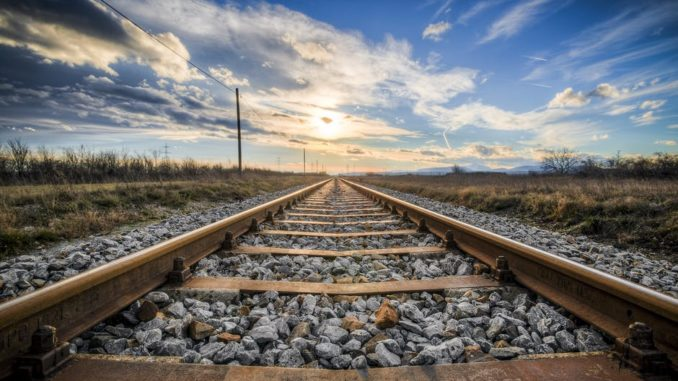
\includegraphics[width=0.5\columnwidth]{1.jpeg}
\end{figure}

\subsection{¿Por qué es necesario usar el plano proyectivo para estudiar las 
transformaciones en las imágenes de fotos de escenas? Dar algún ejemplo.}

% FINISH - To Check - No future

Porque sino no es posible representar traslaciones en un espacio 3D. \newline

En la imagen siguiente y en la de la pregunta anterior vemos ejemplos de proyectivas:

\begin{figure}[h]
	\centering
	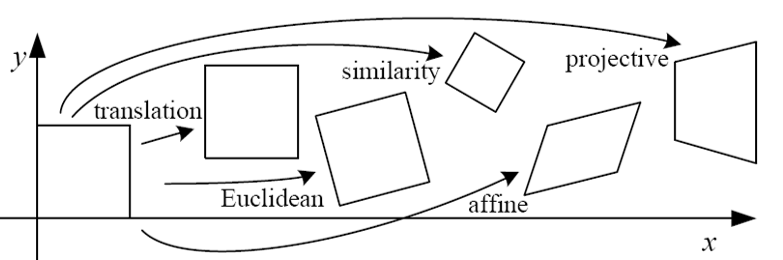
\includegraphics[width=0.7\columnwidth]{5.png}
\end{figure}

\subsection{Sabemos que en el plano proyectivo un punto no existe en el sentido 
del plano afín, sino que se define por una clase de equivalencia de vectores 
definida por {k(x,y,1),k!=0}. Razone usando las coordenadas proyectivas de los 
puntos afines de una recta que pase por el (0,0) del plano afín y verifique que 
los puntos de la recta del infinito del plano proyectivo son necesariamente 
vectores del tipo (*,*,0) con *=cualquier número.}

% FINISH - No future

% Mirar apuntes

Pregunta no contestada

\subsection{¿Qué propiedades de la geometría de un plano quedan invariantes 
cuando se toma una foto de él? Justificar la respuesta.}

% FINISH - To Check

La única propiedad que no es afectada por ninguna transformación es la 
rectitud de las líneas. \newline
Las transformaciones proyectivas, siendo las más disruptivas, no conservan 
ángulos, distancias, orientaciones ni paralelismos.

% --------------------------------------------------------------------------

\subsection{ }
\begin{figure}[h]
	\centering
	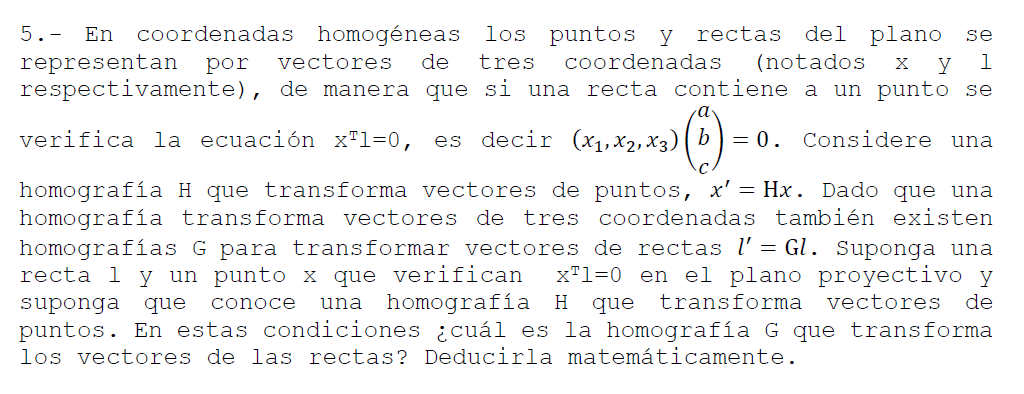
\includegraphics[width=1.0\columnwidth]{p5.png}
\end{figure}

% FINISH - To check

Tenemos que:
\begin{equation}
	x' = H x
\end{equation}
\begin{equation}
	l' = G l
\end{equation}
\begin{equation}
	\begin{aligned}
		det(H) = 0 \\
		det(G) = 0		
	\end{aligned}
\end{equation}
\begin{equation}
	x^{T} l = 0
\end{equation}

Y por tanto:
\begin{equation}
	x'^{T} l' = 0
\end{equation}

Sustituimos $x'$ y $l'$:
\begin{equation}
	(Hx)^{T} l' = 0
\end{equation}
\begin{equation}
	(Hx)^{T} (Gl) = 0
\end{equation}
\begin{equation}
	x^{T} H^{T} G l = 0
\end{equation}

Por la tercera ecuación, tomamos:
\begin{equation}
	H^{T} G = I
\end{equation}

Y nos da:
\begin{equation}
	G = (H^{T})^{-1}
\end{equation}

\subsection{¿Cuál es el mínimo número de escalares necesarios para fijar
una homografía general? ¿Y si la homografía es afín? Justificar la
respuesta}

% FINISH

Para calcular una homografía general es necesario tener como mínimo 8 escalares (4 parejas), 
y forzar a que el determinante de la homografía sea distinto de cero, de forma que
la ecuación:

\begin{figure}[h]
	\centering
	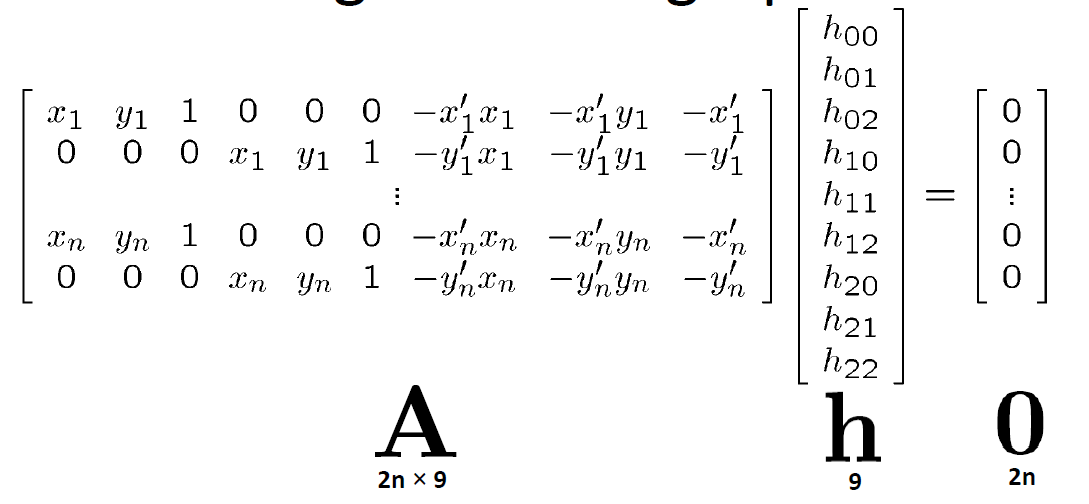
\includegraphics[width=0.5\columnwidth]{6.png}
\end{figure}

al minimizarse con mínimos cuadrados no tenga infinitas soluciones. 
Como resultado obtenemos una matriz de 3x3 con 9 escalares. \newline

Una homografía afín es una donde la última fila de la matriz vale 
$\begin{bmatrix}0 & 0 & 1\end{bmatrix}$, y se define como combinación de una 
transformación lineal y una traslación.
Por tanto son necesarios 6 escalares para fijarla.

\subsection{Defina una homografía entre planos proyectivos que haga que el
punto (3,0,2) del plano proyectivo-1 se transforme en un punto de
la recta del infinito del plano proyectivo-2? Justificar la
respuesta}

% FINISH - To check

Solo es necesario transformarlo en un vector de la forma:
\begin{equation}
	\left( 
		\begin{array}{c}x' \\ y' \\ 0\end{array} 
	\right)
\end{equation}

Por tanto:
\begin{equation}
	\left( 
		\begin{array}{c}a \\ d \\ g\end{array} 
		\begin{array}{c}b \\ e \\ h\end{array} 
		\begin{array}{c}c \\ f \\ i\end{array} 
	\right) *
	\left( 
		\begin{array}{c}3 \\ 0 \\ 2\end{array} 
	\right)
	=
	\left( 
		\begin{array}{c}3a + 2c \\ 3d + 2f \\ 3g + 2i \end{array} 
	\right)
	= 
	\left( 
		\begin{array}{c}x' \\ y' \\ 0\end{array} 
	\right)
\end{equation}

Y podríamos tomar la homografía:
\begin{equation}
	H = 
	\left( 
		\begin{array}{c}a \\ d \\ g\end{array} 
		\begin{array}{c}b \\ e \\ h\end{array} 
		\begin{array}{c}c \\ f \\ i\end{array} 
	\right)
	= 
	\left( 
		\begin{array}{c}0 \\ 1 \\ 0\end{array} 
		\begin{array}{c}1 \\ 1 \\ 1\end{array} 
		\begin{array}{c}1 \\ 1 \\ 0\end{array} 
	\right)
\end{equation}

Que nos daría el punto:
\begin{equation}
	\left( 
		\begin{array}{c}0 \\ 1 \\ 0\end{array} 
		\begin{array}{c}1 \\ 1 \\ 1\end{array} 
		\begin{array}{c}1 \\ 1 \\ 0\end{array} 
	\right) *
	\left( 
		\begin{array}{c}3 \\ 0 \\ 2\end{array} 
	\right)
	=
	\left( 
		\begin{array}{c}2 \\ 5 \\ 0\end{array} 
	\right)
\end{equation}

% --------------------------------------------------------------------------

\newpage

\subsection{ }
\begin{figure}[h]
	\centering
	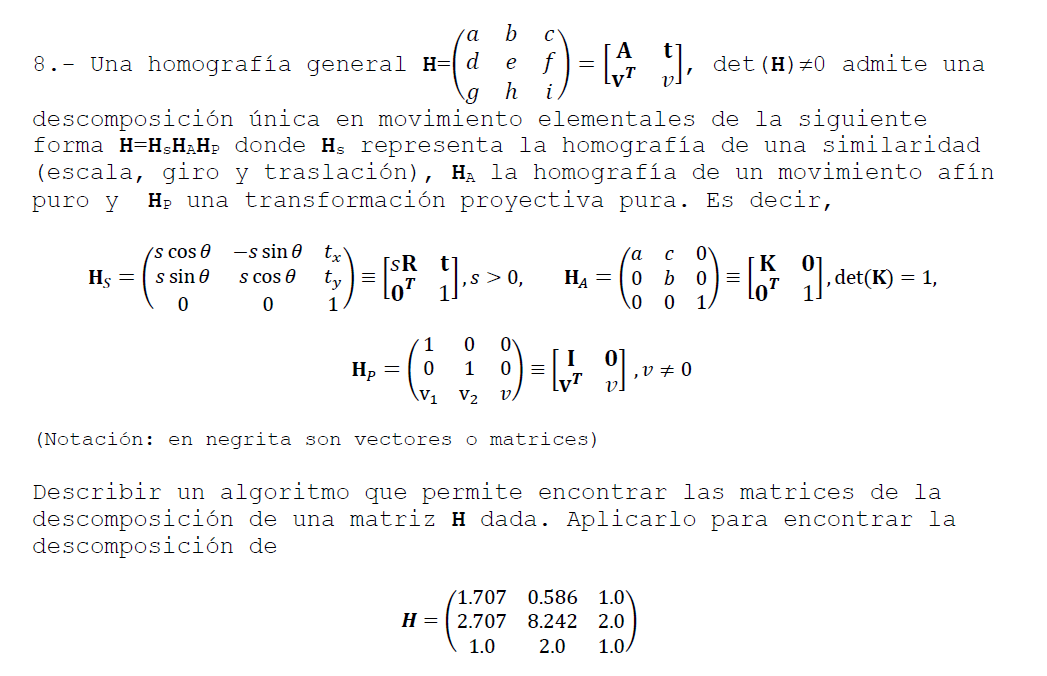
\includegraphics[width=1.0\columnwidth]{p8.png}
\end{figure}

% FINISH

En base al enunciado, tenemos que:
% H.item(8) es v
\begin{equation}
	v = i
\end{equation}
% H.item(6y7) son vT
\begin{equation}
	v^{T} = \begin{bmatrix}g & h\end{bmatrix}	
\end{equation}
% H.item(2y5) son t
\begin{equation}
	t = \begin{bmatrix}c \\ f\end{bmatrix}
\end{equation}
% H.item(0y2y1) son K
\begin{equation}
	K = \begin{bmatrix}a & c \\ 0 & b\end{bmatrix}
\end{equation}

% Para la que nos dan
Esto nos da que:
% Hp = (I 0 / vT v) = (1 0 0 / 0 1 0 / 1.0 2.0 1.0)
\begin{equation}
	H_{P} = \begin{bmatrix}I & 0 \\ v^{T} & v\end{bmatrix} = 
	\left( 
		\begin{array}{c}1 \\ 0 \\ g\end{array} 
		\begin{array}{c}0 \\ 1 \\ h\end{array} 
		\begin{array}{c}0 \\ 0 \\ i\end{array} 
	\right)
\end{equation}


% Ha = (K 0 / 0T 1) = (1.707 1.0 0 / 0 0.586 0 / 0 0 1)
\begin{equation}
	H_{A} = \begin{bmatrix}K & 0 \\ 0^{T} & 1\end{bmatrix} = 
	\left( 
		\begin{array}{c}a \\ 0 \\ 0\end{array} 
		\begin{array}{c}c \\ b \\ 0\end{array} 
		\begin{array}{c}0 \\ 0 \\ 1\end{array} 
	\right)
\end{equation}

% Hs = (sR t / 0T 1) = (? ? 1.0 / ? ? 2.0 / 0 0 1)
\begin{equation}
	H_{S} = \begin{bmatrix}sR & t \\ 0^{T} & 1\end{bmatrix} = 
	\left( 
		\begin{array}{c}s\cos\theta \\ s\sin\theta \\ 0\end{array} 
		\begin{array}{c}-s\sin\theta \\ s\cos\theta \\ 0\end{array} 
		\begin{array}{c}c \\ f \\ 1\end{array} 
	\right)
\end{equation}

En el artículo [\emph{Deeper Understanding of the homography decomposition for
vision-based control}] se explican varios métodos del cálculo de la matriz $R$.
En el propuesto por los autores, se puede obtener en base al vector de traslación
y al vector normal, siguiendo la fórmula:

\begin{figure}[h]
	\centering
	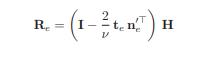
\includegraphics[width=0.35\columnwidth]{9.png}
\end{figure}

\newpage

% Multiplicar, igualar y resolver ecuaciones ??
% Solo dos incógnitas, s y ángulo
% det(H) != 0, s > 0 
% det(K) = 1.707 * 0.586 =(aprox) 1
% v = 1 != 0

% --------------------------------------

Descomponiendo la matriz dada tendríamos:
% H.item(8) es v
\begin{equation}
	v = 1.0
\end{equation}
% H.item(6y7) son vT
\begin{equation}
	v^{T} = \begin{bmatrix}1.0 & 2.0\end{bmatrix}
\end{equation}
% H.item(2y5) son t
\begin{equation}
	t = \begin{bmatrix}1.0 \\ 2.0\end{bmatrix}
\end{equation}
% H.item(0y2y1) son K
\begin{equation}
	K = \begin{bmatrix}1.707 & 1.0 \\ 0 & 0.586\end{bmatrix}
\end{equation}

% Hp = (I 0 / vT v) = (1 0 0 / 0 1 0 / 1.0 2.0 1.0)
\begin{equation}
H_{P} = \begin{bmatrix}I & 0 \\ v^{T} & v\end{bmatrix} = 
\left( 
	\begin{array}{c}1 \\ 0 \\ 1.0\end{array} 
	\begin{array}{c}0 \\ 1 \\ 2.0\end{array} 
	\begin{array}{c}0 \\ 0 \\ 1.0\end{array} 
\right)
\end{equation}


% Ha = (K 0 / 0T 1) = (1.707 1.0 0 / 0 0.586 0 / 0 0 1)
\begin{equation}
H_{A} = \begin{bmatrix}K & 0 \\ 0^{T} & 1\end{bmatrix} = 
\left( 
	\begin{array}{c}1.707 \\ 0 \\ 0\end{array} 
	\begin{array}{c}1.0 \\ 0.586 \\ 0\end{array} 
	\begin{array}{c}0 \\ 0 \\ 1\end{array} 
\right)
\end{equation}

% Hs = (sR t / 0T 1) = (? ? 1.0 / ? ? 2.0 / 0 0 1)
\begin{equation}
	H_{S} = \begin{bmatrix}sR & t \\ 0^{T} & 1\end{bmatrix} = 
	\left( 
		\begin{array}{c}s\cos\theta \\ s\sin\theta \\ 0\end{array} 
		\begin{array}{c}-s\sin\theta \\ s\cos\theta \\ 0\end{array} 
		\begin{array}{c}1.0 \\ 2.0 \\ 1.0\end{array} 
	\right)
\end{equation}

\subsection{¿Cuáles son las propiedades necesarias y suficientes para que
una matriz defina un movimiento geométrico no degenerado entre
planos? Justificar la respuesta}

% FINISH

Pregunta no contestada.

\subsection{¿Qué información de la imagen usa el detector de Harris para
seleccionar puntos? ¿El detector de Harris detecta patrones
geométricos o fotométricos? Justificar la contestación.}

% FINISH - TO CHECK - No future

Harris utiliza los gradiendes de una zona local al píxel para seleccionar los 
puntos. Observando los cambios de intensidad de las esquinas, es capaz de detectar
patrones geométricos siendo invariante a traslaciones y rotaciones. \newline

También es capaz de detectar algunos patrones fotométricos al ser parcialmente
invariante a cambios de intensidad, generalmente a aquellos débiles.

% Harris detecta patrones geométricos

% (USA LOS GRADIENTES, las derivadas ??)

% Detecta patrones geométricos, pero calcula fotométricos (al estar basado en la
% intensidad de los píxeles)

% (IMAGEN CAMBIO DE INTENSIDAD ?)

% Del PDF
% La información que utiliza el detector de Harris para seleccionar puntos es el
% cambio de intensidad en varias direcciones existentes entre ellos.
% Puede detectar patrones geométricos, ya que es capaz de encontrar las esquinas de 
% objetos geométricos y patrones fotométricos, ya que propiamente utiliza los cambios
% de la intensidad, aunque no sean zonas con objetos geométricos.

\subsection{¿Sería adecuado usar como descriptor de un punto Harris los
valores de los píxeles de su región de soporte? Identifique
ventajas, inconvenientes y mecanismos de superación de estos
últimos.}

% FINISH - No future

No, porque aunque sea fácil de calcular, queremos usar como descriptor algo
que sea invariante a transformaciones afines y proyectivas. \newline

Los gradientes cumplen esta propiedad, pero los valores de los píxeles se ven 
afectados por transformaciones, como orientaciones y escalas.


% Del PDF
% Para usar como descriptor de  un punto Harris los valores de los píxeles de su
% región de soporte se tiene que comprobar que la relación entre los píxeles de esa
% región no varía al aplicar las transformaciones.
% Si se aplica una traslación, los puntos al final mantienen la misma estructura que 
% antes de realizar la transformación. Aplicando una rotación, escalado, cizalla o
% proyección, los puntos ya no mantienen la misma relación entre sí, por lo que ya no
% es adecuado usarlos como descriptor de un punto.

\newpage

\subsection{Describa un par de criterios que sirvan para seleccionar
parejas de puntos en correspondencias (“matching”) a partir de
descriptores de regiones extraídos de dos imágenes. ¿Por qué no es
posible garantizar que todas las parejas son correctas?}

% FINISH - TO CHECK

Hemos tratado con dos criterios:
\begin{enumerate}
	\item \textbf{Fuerza bruta junto a CrossCheck}: 
	% Elegimos el mínimo por filas y por 
	% columnas. Esto quiere decir que cogemos aquellas parejas de puntos que se
	% tienen mutuamente el uno a otro como el de menor distancia.
	Este criterio elige para cada descriptor de la primera imagen aquél más 
	cercano en la segunda y viceversa. Si ambas parejas coinciden, se almacena 
	como una correspondencia final.
	\item \textbf{Criterio de Lowe}: Para cada punto en la primera imagen elegimos los dos
	a menor distancia en la segunda. Sí la distancia entre estos dos puntos está por debajo de
	un cierto ratio se añade el punto y el de menor distancia como correspondencia.
\end{enumerate}

En imágenes con ambigüedad los criterios tienen problemas para garantizar
que las parejas son correctas.
Esto se debe a que los descriptores SIFT realizan un cálculo local al píxel y
en ciertas imágenes (como la de abajo) esto puede generar distancias muy similares.

\begin{figure}[h]
	\centering
	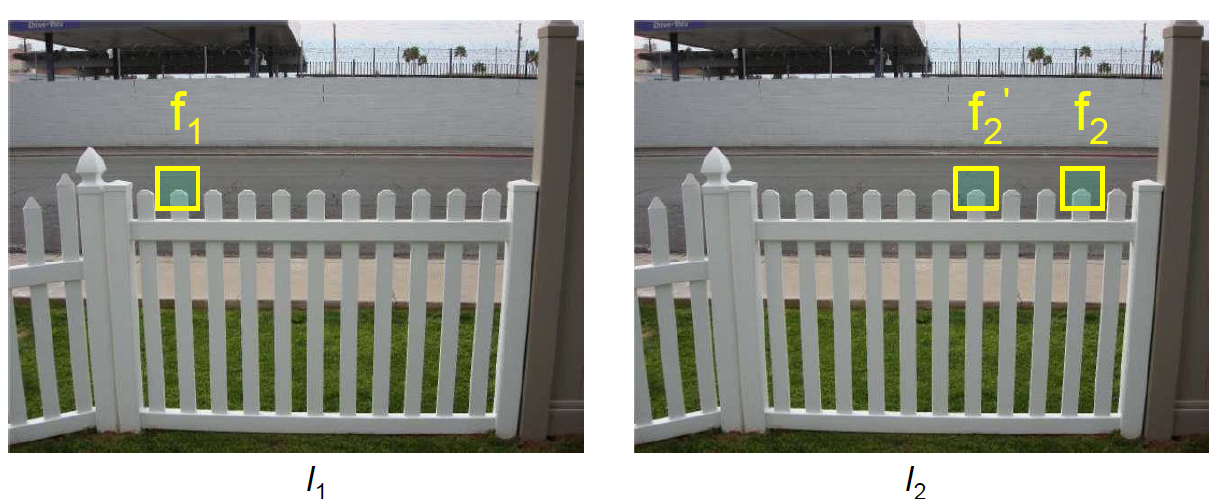
\includegraphics[width=1.0\columnwidth]{1.png}
\end{figure}


\subsection{Cual es el objetivo principal del uso de la técnica RANSAC en
el cálculo de una homografía. Justificar la respuesta}

% FINISH - TO CHECK

El objetivo es la obtención de una homografía de mejor calidad.
En la pregunta anterior se ha visto que existen casos en los que los criterios de 
correspondencias no pueden asegurar que las parejas sean correctas. Estos errores
empeoran en gran medida la calidad de la homografía, ya que al estar calculando mínimos 
cuadrados las correspondencias erróneas alteran el resultado.

\begin{figure}[h]
	\centering
	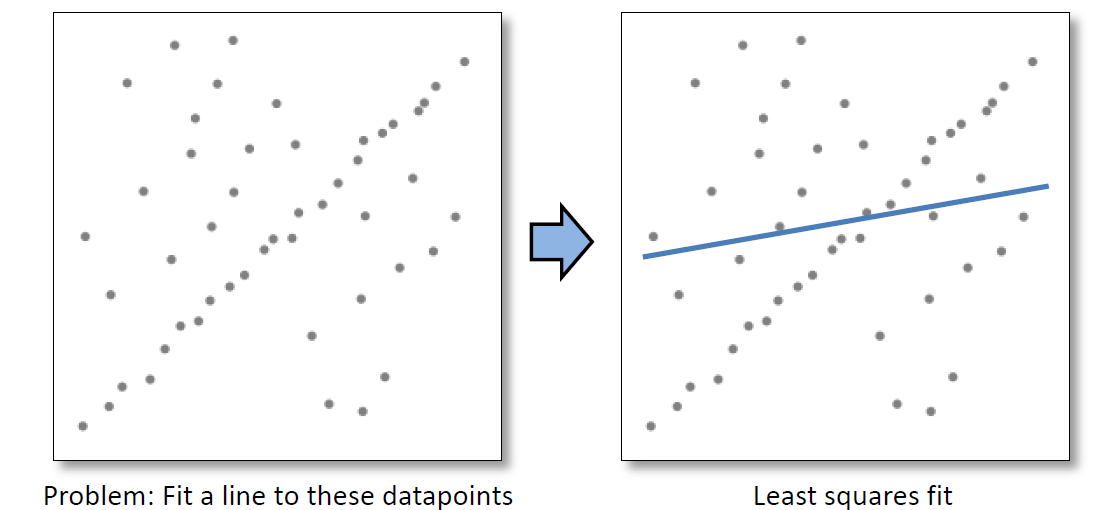
\includegraphics[width=1.0\columnwidth]{2.png}
	\caption{Problema de mínimos cuadrados}
\end{figure}

Con RANSAC pretendemos seleccionar la homografía que adapta en buena manera la 
mayor cantidad de puntos posibles, ignorando el resto. \newline

El algoritmo muestrea 4 parejas de puntos, calcula la homografía asociada, y 
calcula la cantidad de correspondencias que se ajustan a ella de manera correcta
(en base a un parámetro variable). Tras un número de iteraciones elige aquella 
homografía con la mayor cantidad de parejas a su favor.

\subsection{Si tengo 4 imágenes de una escena de manera que se solapan la
1-2, 2-3 y 3-4. ¿Cuál es el número mínimo de parejas de puntos en
correspondencias necesarios para montar un mosaico? Justificar la
respuesta}

% FINISH - TO CHECK

12 parejas. \newline 
Puesto que necesitamos 3 homografías, y el número de parejas mínimo para una 
homografía es 4. \newline

Se definiría manualmente una homografía inicial para fijar una de las 
imágenes, se calcularían las 3 homografías usando las 4 parejas en cada una
(1-2, 2-3 y 3-4), 
y mediante composición de homografías se iría construyendo el mosaico.


% 3 homografías con mínimo 4 parejas por cada una -> 12 parejas
% Mínimo 4 parejas porque nos definen ... EXPLICAR LO DE LAS INFINITAS SOLUCIONES

% Se definiría manualmente una homografía inicial para fijar una de las 
% imágenes, se calcularían las 3 homografías usando las 4 parejas en cada una,
% y mediante composición de homografías se iría construyendo el mosaico.

\subsection{¿En la confección de un mosaico con proyección rectangular es
esperable que aparezcan deformaciones geométricas de la escena
real? ¿Cuáles y por qué? ¿Bajo qué condiciones esas deformaciones
podrían no estar presentes? Justificar la respuesta.}

% FINISH - To check - No future

En clase hemos visto deformaciones geométricas y una fotométrica.
% (alargamientos y problemas de colores)

Sobre las geométricas, en la construcción de mosaicos calculamos las homografías 
y proyectamos sobre un plano rectangular. 
Esto genera distorsiones en los laterales de los mosaicos.
Debidas a que estamos proyectando imágenes rotadas en un espacio 
tridimensional sobre un mismo plano. \newline

La solución a este tipo de problemas sería generar el mosaico sobre un espacio
cilíndrico o esférico, donde se proyectarían las imágenes a igual tamaño sobre 
la superficie. \newline

% Imagen
\begin{figure}[h]
	\centering
	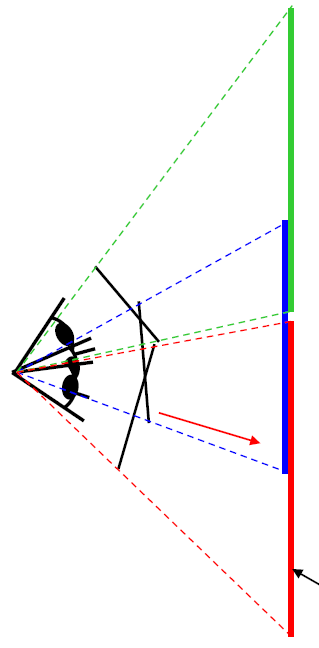
\includegraphics[width=0.2\columnwidth]{3.png}
	\caption{Proyectando sobre un plano}
\end{figure}

% Efectos deformaciones - ESTA NO TIENE DEFORMACIONES en los laterals
\begin{figure}[h]
	\centering
	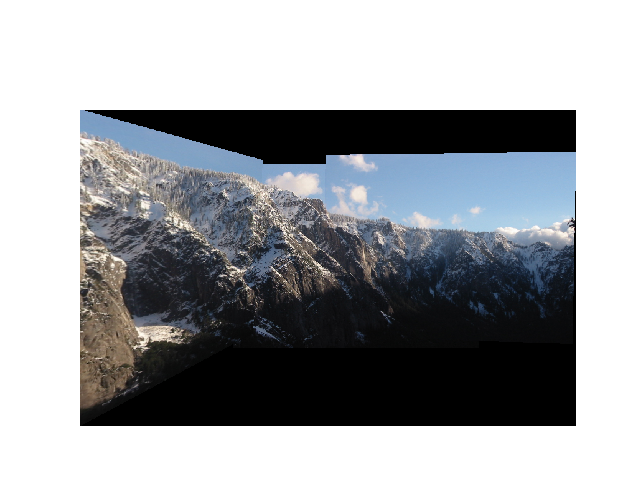
\includegraphics[width=0.7\columnwidth]{8c.png}
	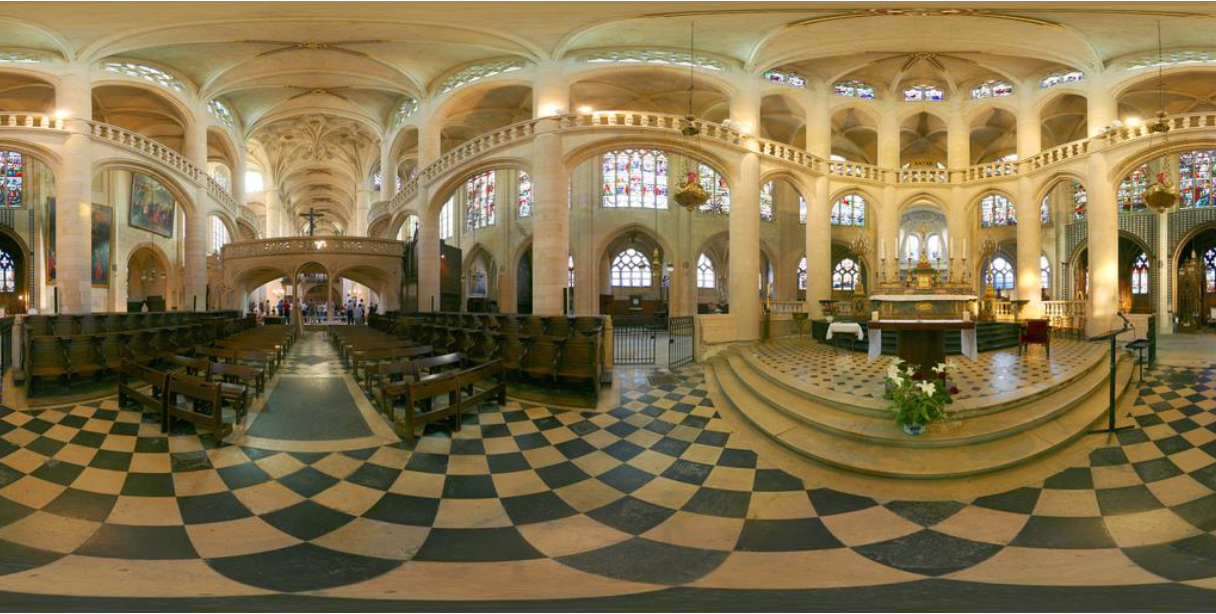
\includegraphics[width=0.7\columnwidth]{4.png}
	\caption{Deformaciones de los mosaicos}
\end{figure}

Otro problema que se origina es la acumulación de pequeños errores a lo largo del mosaico, que
emperoran la forma de la imagen.

\end{document}